\subsection{Automaten}
Es wurde versucht Automaten sowohl möglichst nah an der theoretischen Vorgabe als auch möglichst effizient zu implementieren. Daraus hat folgende Grundimplementation resultiert.
\begin{figure}[h]
  \centering
  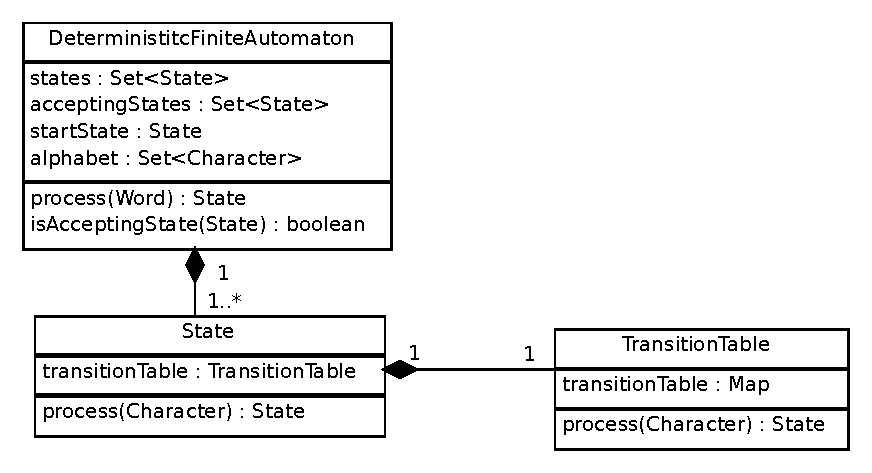
\includegraphics[width=0.5\textwidth]{images/dfa_classdiag_simple.pdf}
  \caption[DFA Klassendiagramm vereinfacht]{DFA Klassendiagramm vereinfacht}
  \label{fig:dfa_classdiag_simple}
\end{figure}

Das Quintupel ($Q$, $\Sigma$, $\delta$, $q0$, $F$) ist darin wie folgt abgebildet:

\begin{table}[h]
  \centering
  \begin{tabular}{ l | l }
    \hline
    $Q$ & Die Menge der Zustände wurde als Set von States implementiert.  \\
    \hline
    $\Sigma$ & Das Alphabet ist ein Array von Zeichen (Character). \\
    \hline
    $\delta$ & Die Übergangsfunktion $\delta$ wird als Map (Zeichen -> Zustand) 
    \\ & auf den einzelnen Zuständen abgebildet. Dies erlaubt uns eine
    \\ & einfache und effiziente Verarbeitung von Eingaben sowohl auf
    \\ & Zustands als auch auf Automaten Ebene. \\
    \hline
    $q0$ & Eine Referenz zum Startzustand $q0$ ist in der DFA Klasse hinterlegt. \\
    \hline
    $F$ & Die Menge der Akzeptierenden Zustände wird durch ein Set auf dem \\ & jeweiligen DFA Objekt representiert. \\
    \hline 
  \end{tabular}
  \caption[Implementation Automaten]{Implementation automaten}
\end{table}

Ein solcher Automat kann nun mithilfe seiner \lstinline$process(Word)$ Funktion ein Wort (Eine Liste von Zeichen) verarbeiten indem er sich die Referenz des ersten Zustandes \lstinline$startState$ holt und dann Zeichen für Zeichen jeweils mit \lstinline$process(Character)$ die Referenz des nächsten Zustandes herausliest. Zurückgegeben wird schlussendlich derjenige Zustand der am Ende der verarbeiteten Zeichenkette erreicht wurde. Mithilfe der \lstinline$isAcceptingState(State)$ Methode kann festgestellt werden ob das Wort akzeptiert wird oder nicht. 

Zum besseren Verständnis folgend die \lstinline$process$ Methode der DFA Klasse als Pseudocode:

\begin{lstlisting}[language=Python, caption={Process Methode der DFA Klasse}]
def process(word):
  state = startState
  for char in word:
    state = state.process(char)
  return state
\end{lstlisting}

\paragraph{Visualisierung}
Zur Visualisierung der Automaten wurde Graphviz \cite{graphviz} mit dem Graphviz Java API \cite{graphvizjava} verwendet. Konkret wurde ein Interface \lstinline$GraphvizRenderable$ entwickelt welches Klassen vorschreibt die \lstinline$generateDotString()$ Methode zu implementieren.

In der statischen Klasse \lstinline$GraphvizRenderer$ wurde eine Methode \lstinline$renderGraph(GraphvizRenderable, FileName)$ implementiert welche das API ansteuert und das gegebene \lstinline$GraphvizRenderable$ Objekt als SVG Vektorgraphik abspeichert.

Damit das generieren der Grafiken funktioniert, muss die \lstinline$generateDotString()$ Methode eine gültige Graphviz DOT Graphbeschreibung als String zurückgeben. Automaten sind eine Form von Digraphen und können in der DOT Sprache wie folgt beschrieben werden:

\begin{lstlisting}[language=Java, caption={Automat in DOT Sprache}, label={lst:dot_language}]
digraph G {
  q0 -> q1 [label="0"]
  q0 -> q2 [label="1"]
  q1 -> q2 [label="0"]
  q1 -> q0 [label="1"]
  q2 -> q0 [label="0"]
  q2 -> q1 [label="1"]
  q2 [peripheries=2]
  q0 [color=darkred]
}
\end{lstlisting}

\begin{itemize}
  \item \lstinline$digraph G$ definiert den Graphentypen
  \item \lstinline$q0 -> q1$ definiert den Übergang vom Knoten \lstinline$q0$ auf den Knoten \lstinline$q1$
  \item \lstinline$[label="0"]$ fügt die Beschriftung \flqq 0\frqq dem Übergang hinzu
  \item \lstinline$[peripheries=2]$ umrandet den entsprechenden Knoten doppelt
  \item \lstinline$[color=darkred]$ färbt den entsprechenden Knoten dunkelrot ein
\end{itemize}

Eine Anleitung zur DOT Sprache ist in den Quellen verlinkt. \cite{graphvizdotref}

\paragraph{Überprüfen von Automaten}
Um beim zufälligen mutieren und rekombinieren der Automaten prüfen zu können, ob ein Automat die selbe Sprache akzeptiert wie der gegebene reguläre Ausdruck, wurde das Java Package \lstinline$dk.brics.automaton$ von der dänischen Aarhus Universität verwendet.\cite{bricsautomaton}

In diesem Package sind verschiedene Algorithmen rund um endliche Automaten implementiert. Unter anderem kann es einen Automaten aus einem regulären Ausdruck erzeugen und verschiedene Automaten darauf überprüfen ob sie die selbe Sprache akzeptieren. Die Umwandlung von einem Automaten unserer Implementation in einen \lstinline$dk.brics.automaton$ wurde im Package \lstinline$ch.zhaw.regularLanguages.dfa.transformation$ implementiert. Es enthält ein Interface \lstinline$Transformer<S, T>$ welches die Methode \lstinline$T transform(S input)$ vorschreibt und die konkrete Implementation \lstinline$TransformDFAToBricsAutomaton$ welches die Transformation von unserem DFA in einen \lstinline$dk.brics.automaton.Automaton$ beherrscht. Die Umwandlung läuft wie folgt ab:
\begin{enumerate}
  \item Leerer \flqq BRICS Automat\frqq wird erzeugt
  \item Für jeden unserer Zustände wird dem Automaten einen Zustand hinzugefügt
  \item Die Übergangstabelle wird übertragen
  \item Akzeptierende Zustände werden entsprechend markiert
  \item Startzustand wird gesetzt
\end{enumerate}

\paragraph{Vereinfachung}
Zur Erhöhung der Konsistenz von Automaten, wurde eine Methode zum entfernen aller nicht erreichbaren Zustände implementiert. Insbesondere verhindert dies eine \flqq Aufsplittung\frqq wie sie in Abbildung \ref{fig:split_dfa} zu sehen ist. In diesem Beispiel gibt es keine Verbindung vom Startzustand $q0$ zum einzig akzeptierenden Zustand $q4$.

\begin{figure}[H]
  \centering
  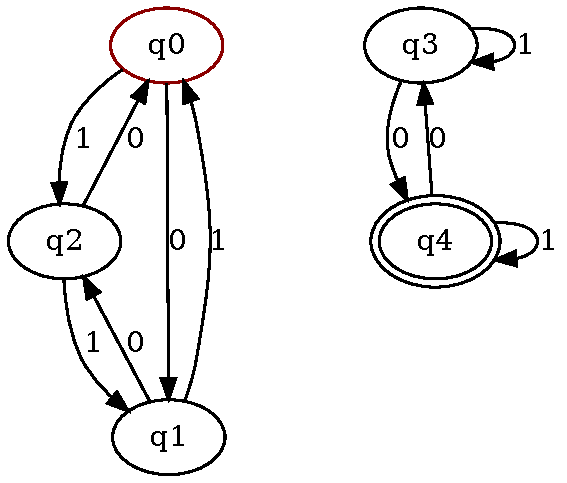
\includegraphics[width=0.5\textwidth]{images/split_automaton.pdf}
  \caption[Aufgesplitteter Automat]{Aufgesplitteter Automat}
  \label{fig:split_dfa}
\end{figure}

In der Methode zum entfernen der nicht erreichbaren Zustände werden vom Startzustand aus alle möglichen Verbindungen getestet. Jene Zustände die so nicht erreicht werden können werden entfernt. Zum besseren Verständnis ist folgend die Methode als in Python-Pseudocode dokumentiert.  

\begin{lstlisting}[language=Python, caption={Algorithmus zum entfernen von nicht erreichbaren Zuständen}, label={lst:remove_unreachable_states}]
def removeUnreachableStates(dfa):
  processed = []
  current = dfa.getStartState()
  queue = [current]
  
  while queue.size > 0:
    nextList = []
    for char in dfa.getAlphabet():
      nextList.append(current.process(char))

    processed.append(current)
    queue.remove(current)

    for nextState in nextList:
      if !processed.contains(nextState):
        queue.append(nextState)

    current = queue[0]

  newStates = processed
  dfa.setStates(newStates)
\end{lstlisting}

\subsubsection{RandomDeterministicFiniteAutomaton}
\label{subsec:RandomDeterministicFiniteAutomaton}
Der \lstinline$RandomDeterministicFiniteAutomaton$ ist eine Erweiterung für unsere DFA Klasse, welche den normalen endlichen Automaten um einen zufälligen Konstruktor und eine \lstinline$mutate$ Methode zum zufälligen mutieren des Automaten erweitert.

\paragraph{Der Konstruktor} erzeugt mithilfe eines gegebenen Alphabets und einem Faktor für die Komplexität des Problems - wie folgt beschrieben - zufällige Automaten.
\begin{enumerate}
  \item Es wird eine Menge von Zuständen erzeugt (Anzahl Zustände: zwischen $1$ und $(2 \cdot AnzahlZeichen \cdot Komplexitaet)$ wobei $AnzahlZeichen$ die Anzahl der Zeichen des Alphabets und die $Komplexität$ ein Faktor ist welcher als Parameter an den Konstruktor übergeben wird).
  \item Jedem Zustand werden für jedes Zeichen des Alphabets zufällig Verbindungen auf andere Zuständen zugeordnet.
  \item Der erste Zustand (q0) wird zum Startzustand.
  \item Um sicherzustellen dass jeder Automat erreichbare akzeptierende Zustände hat, werden alle nicht erreichbaren Zustände entfernt.
  \item Eine zufällige Menge von Zuständen (zwischen $1$ und $\frac{AnzahlZustaende}{5}$) wird zu akzeptierenden Zuständen.
\end{enumerate}

\paragraph{Die \lstinline$mutate$ Methode} greift auf ein Mutationsregister zurück in welchem die Methoden zum Verändern von Automaten registriert sind. Dabei wählt es zufällig eine Methode aus und führt diese durch. Wenn die Mutation erfolgreich war sind wir fertig. Wenn nicht wird erneut eine zufällige Methode ausgesucht. Dies wird solange wiederholt bis der Automat erfolgreich verändert wurde.

\begin{center}
  \begin{tabular}{| l | p{7cm} | p{4cm} |}
    \hline
    \textbf{Aktion} &  \textbf{Beschreibung} & \textbf{Bedingungen}\\
    \hline
    Zustand hinzufügen 
    & Es wird ein Zustand zum Automaten hinzugefügt. Für jedes Zeichen im Alphabet wird ein Übergang auf einen zufälligen Zustand des Automaten gelegt. Danach wird berechnet wieviele Verbindungen in diesem Automaten durchschnittlich zu einem Zustand führen ($avg$). Mit diesem Resultat werden zwischen $\frac{avg}{2}$ und $avg \cdot 2$ zufällig ausgewählte Verbindungen von zufällig ausgewählten Zuständen zum neuen gelegt.
    & - \\
    \hline
    Zustand entfernen
    & Es wird zufällig ein Zustand ausgewählt und entfernt. Alle Übergänge die auf diesen Zustand zeigen werden zufällig auf andere Zustände umgeleitet.
    & Nicht der letzte Zustand; Nicht der letzte akz. Zustand \\
    \hline
    Akz. Zustand hinzufügen
    & Es wird ein zufälliger nicht akzeptierender Zustand ausgewählt. Dieser wird zum akzeptierenden Zustand gemacht.
    & Nicht akzeptierende Zustände vorhanden \\
    \hline
    Akz. Zustand entfernen
    & Es wird ein zufälliger akzeptierender Zustand ausgewählt. Dieser wird zu einem regulären nicht-akzeptierenden Zustand umgewandelt.
    & Nicht der letzte akz. Zustand \\
    \hline
    Übergang ändern
    & Es wird ein zufälliger Zustand und ein zufälliges Zeichen ausgewählt. Der abgehende Übergang für das gewählte Zeichen wird zufällig auf einen anderen Zustand gelegt.
    & - \\
    \hline 
  \end{tabular}
  \captionof{table}{Mutationen}
\end{center}

